\documentclass[12pt,twocolumn,letterpaper,Times New Roman]{article}

\usepackage[pagenumbers]{cvpr}
\usepackage{graphicx}
\usepackage{amsmath}
\usepackage{amssymb}
\usepackage{booktabs}
\usepackage[pagebackref,breaklinks,colorlinks]{hyperref}
\usepackage[capitalize]{cleveref}
\crefname{section}{Sec.}{Secs.}
\Crefname{section}{Section}{Sections}
\Crefname{table}{Table}{Tables}
\crefname{table}{Tab.}{Tabs.}

\begin{document}
\title{Image Based Personalized Product Recommendation using Deep Learning}

\author{Kushajveer Singh\\
University of Georgia\\
{\tt\small ks56866@uga.edu}
\and
Vipul Shinde\\
University of Georgia\\
{\tt\small vs85145@uga.edu}
}
\maketitle

\begin{abstract}
Recommendation systems have been the standard method of recommending products used by e-commerce websites. These recommendation systems use previous user-purchase history or item features to recommend products to a user. But for recommending fashion items, the visual appearance of the recommended product must also be taken into consideration, which is often ignored in these recommendation systems. In this paper, we present a two-stage fashion recommendation system which recommends similar items to users based on the image of one of their previous purchase. Our framework consists of a convolutional neural network for extracting the image features and then using the image embeddings to find similar products using the Approximate Nearest Neighbors (annoy) algorithm. We used a publicly available dataset from Kaggle which was scraped from an Indian e-commerce website. The product category classification model was able to achieve an accuracy of 91\% and an AUC score of 0.996 on the validation dataset and we conducted experiments showing how this can be used to recommend similar products to a user. 
\end{abstract}

\textbf{Keywords}: recommendation system, e-commerce, fashion, transfer learning, convolutional neural network, annoy

\section{Introduction}
Revenue made from the sale of recommended items is one of the major revenue streams for most of the major e-commerce websites. This provides a large incentive to cater the recommendations to each user which in turn can significantly increase the earnings of a company. On the other hand, recommending too many items can also be a downside as the user will not be able to locate the specific item of interest. So we want to minimize the number of recommendations while at the same time maximizing the relevance of the recommended items. This can also increase the likelihood of the customer returning to the e-commerce website for making future purchases, thus making the customer a permanent customer, which is a key factor to the profitability of a company.

Image similarity is used in google reverse image search where, similar images are shown for the input image, along with similar keywords. This can also be used for exploration, where we use an image to find similar keywords to search for the products in the image. It has also been used in landmark recognition, where images of the same landmark from different angles can be grouped.

Most of the prior studies focus on recommending products based on a recommendation system based on previous user purchases or item features. But one of the key factors when it comes to recommending fashion based items to a user is the visual similarity of the product to the previous purchases made by the user. The conventional recommendation systems do not take this image similarity into consideration. In this paper, we focus on solving this particular problem, where we want to identify similar images to a given image and then use these images for product recommendation.

To recommend visually similar images our framework consists of two parts. First, a convolutional neural network (CNN) based feature extractor that is used to embed the images into a smaller latent space. To train this model, we used image classification to predict the products into the given categories. This has the advantage that visually similar images would belong to the same category and thus, their latent embeddings would also be closer to each other. After training an image classification model, we used the convolutional base to extract the image embeddings and pass these embeddings downstream to a clustering algorithm. To compare two images a quantitative measure like cosine similarity is used, which would give a score between 0 and 1, like 0.974 which means the two images are 97.4\% similar.

A clustering algorithm is used to group similar images together. As shown in Fig \ref{fig:fig1} similar content can mean different things. Maybe two images have similar content but have different resolution, or if the image is translated or rotated or if the color histogram of the image is shifted or if the style of the image is different. As we can see there is a lot of ambiguity about what is considered a similar image. And as a result of this, the similar images must appear closer to each other in the embedding space. Now to find the closest images in this space, a clustering algorithm like Approximate Nearest Neighbors (annoy) is used.

\begin{figure*}
  \centering
  \begin{subfigure}{0.4\linewidth}
    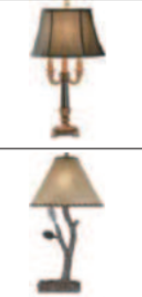
\includegraphics[height=4cm]{images/fig1.png}
    \caption{Image of two different lamps.}
  \end{subfigure}
  \begin{subfigure}{0.4\linewidth}
    
\includegraphics[height=4cm]{images/fig2.png}
    \caption{Images of mario but with different style}
  \end{subfigure}
  \caption{Similar content can be independent of resolution, translation, rotation, color and style. As shown in (a) both images are of a lamp but we can clearly see the differences in the image. In (b) both images are of mario but the first image is a pixelated image and the second image if a high-definition image. In this context, both have the same content but their style is different.}
  \label{fig:fig1}
\end{figure*}

Our contributions are two-fold. (i) We train an image classification model which learns to group similar images together by using the downstream task of image classification. (ii) Image embeddings from CNN are clustered together by Annoy which is used to output similar images.

\section{Related Work}
\textbf{Recommendation system}. The two main approaches for product recommendation include collaborative filtering and content-based filtering. In collaborative filtering, a database of user ratings is maintained which is then used to recommend similar products to users based on similar ratings. In content-based filtering, the recommendations are based on the content of the items rather than on the user features. Therefore, this method uses item features to recommend other similar items to what a user would like. While recommending fashion items both the methods ignore the image features.

\textbf{Pixel comparison}. Comparing images pixel by pixel cannot be used to solve this problem. The main limitation of this approach is that we do not get translational and rotational invariance. As a result, if the item in the image is slightly shifted to the right, this method would give bad results.

\textbf{Keypoint detection}. This technique comes from facial detection, where we can identify various keypoints on a human face and then process the images based on these features, so find similar faces. The main drawback of this approach is that it requires a lot of domain knowledge and for millions of products on the e-commerce websites it is not practical to construct keypoint for each product.

\textbf{Color distribution}. Color histogram of two images can be compared to check how similar the images are. However this method is not invariant to color changes. Same product can have different colors and this method would classify them as different products.

\textbf{Linear Discriminant Analysis}. Techniques like PCA \cite{pca} and LDA \cite{lda} are very popular in machine learning. PCA is used to find the features of the data that explain most of the variation of the data. LDA on the other hand is used to separate the data into categories, when projecting into a lower dimension. Therefore, LDA can be used to group similar images together. But a limitation of this approach is that the image features are very high dimensional and curse-of-dimensionality strikes in and makes training a machine learning classifier difficult.

\section{Method}
We propose a two-stage fashion recommendation system. In the first stage, a Convolutional Neural Network (CNN) is trained using transfer learning to classify a given product image into its category \cite{Tuinhof_2019}. Xception \cite{exception} model architecture with pre-trained weights from the ImageNet dataset \cite{imagenet}. The trained CNN model’s Global Average Pooling layer’s output will be used as feature embeddings for the image. Further on, in the second step, we pass on these embeddings to the Approximate Nearest Neighbors (annoy) algorithm. Given an input image, we calculate the image embeddings for it using the CNN and pass it to annoy for calculating the top k nearest similar fashion products. 

Image data provides a lot of information on the visual appearance of a product e.g., edges and color blobs.\cite{prince2012computer} Plenty of image processing techniques exist to extract such low-level features. Deep learning provides an approach to extract these features by using several convolutional layers\cite{Zhang_2020}. Therefore, we have used a CNN for our problem and unlike other conventional techniques for recommendations which rely on user past purchases or history or the item features, we depend solely on the visual features of fashion product.

\begin{figure}[!ht]
    \centering
    % \captionsetup{justification=centering,margin=2cm}
    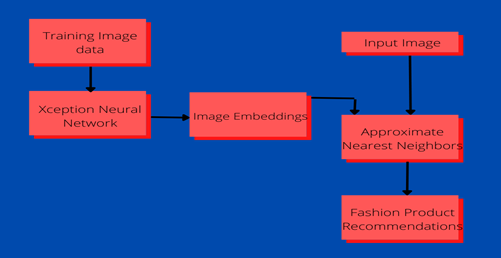
\includegraphics[width=80mm]{fig_7.png}
    \caption{Proposed Machine Learning framework architecture.}
    \label{fig:10}
\end{figure}


\subsection{CNN}
For the image classification model, we used a pre-trained Xception model which is a lightweight model while giving higher accuracy than related models. The convolutional block consisted of a convolution layer, followed by batch normalization, Relu activation and pooling layer. Due to the limitations of the dataset size, an Xception model trained on Imagenet was used.

Xception model proposed depthwise separable convolution, which works by splitting the convolution kernel into two one-dimensional kernels with far less parameters. This results in savings of over 20x the number of parameters, which results in faster training and faster inference.

\subsection{Approximate Nearest Neighbors (annoy)}
In order to calculate exact nearest neighbors most of the times, the algorithms used are exhaustive search. K Nearest neighbors is one of the techniques that is used most often. But since it uses exhaustive search approach, the distance of a given point needs to be calculated from all the other points in the search space. This approach could be solved in linear time i.e., O(n) and if the dataset is huge, this approach is not optimal.

This makes the exact nearest neighbors impractical to use in some cases and the approximate nearest neighbors can capitalize on it. A similarity search can be of orders of magnitude faster if we’re willing to trade some accuracy. Here are a couple of examples where the use of ANN seems like a good idea\cite{trabelsi}:

\begin{itemize}
  \item \textit{Image Search}: If someone is looking for a picture of an ant, it wouldn't matter to them which ant pictures show up.
  \item \textit{Fashion Recommendation}: Similarly, if someone is looking for a t-shirt they wouldn't’t mind if it’s not exact match to the given input image.
\end{itemize}

One of the tree-based ANN algorithms out there is Annoy, which is built and used by Spotify for song recommendations. The time complexity for finding nearest neighbors is reduced to 
O (log N) as we are getting rid of half of the data points every time, we traverse down the tree. The algorithm is called Annoy\cite{erikbern} and is mentioned below:

\begin{enumerate}
  \item Randomly select two data points and then split by the hyperplane equidistant from those two points. 
  \item Keep doing this until we have reached at most k number of samples in each region.
  \item Plot a binary tree out of it. If the points lie below the separating lines, they’ll go in the left node of the tree and vice-versa.
  \item Given a new sample, traverse down the tree and only compute cosine distance with other points in the last node.
\end{enumerate}

\begin{figure}[!h]
    \centering
    % \captionsetup{justification=centering,margin=2cm}
    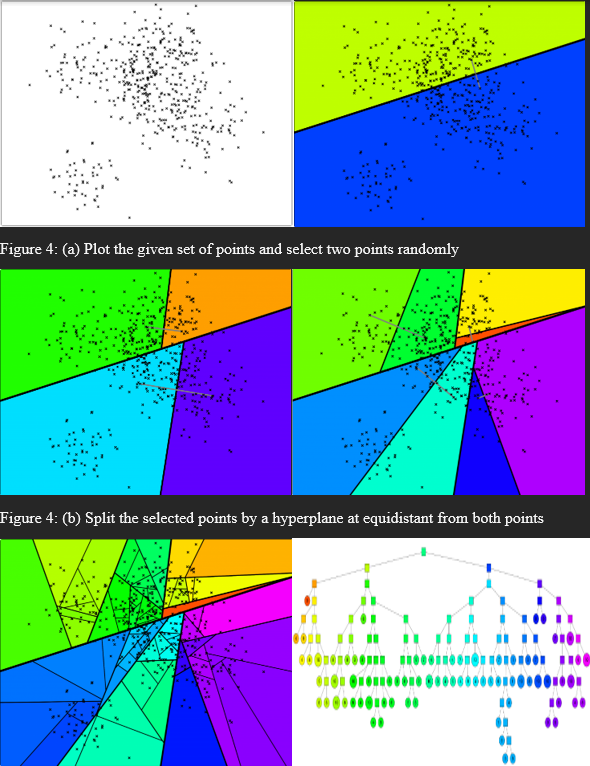
\includegraphics[width=80mm]{fig_4.png}
    \caption{(c) Keep splitting until k number of samples remain in each plane and plot the binary tree}
    \label{fig:11}
\end{figure}

We take the image embeddings from the Global Average Pooling layer of our CNN model and use it as our search space. When the user provides an input image, we use the CNN to infer its embeddings which then is provided as an input to the Annoy algorithm. The ANN algorithm will then search the space and give the top k approximate recommendations for the given fashion product.

\section{Experiments}

\subsection{Dataset}

We will be using a subset of the publicly available dataset on Kaggle. Originally, the product images were scraped from an e-commerce website. Our data consists of in total 12,000 images of fashion products from top 8 different categories. (1500 each) 

The class labels for the category types are Shirts, Watches, Casual shoes, Kurta, Sport shoes, Tops, T-shirts and Handbags. The below figure shows the total number of images across top 8 different categories from the original dataset. Along with the image data, we also have the metadata containing other product features such as name, gender, color, etc.

\begin{figure}[!h]
    \centering
    % \captionsetup{justification=centering,margin=2cm}
    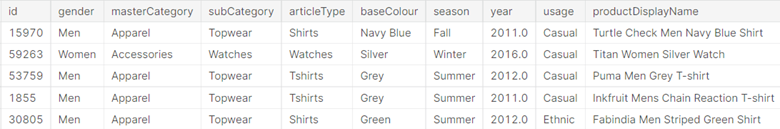
\includegraphics[width=80mm]{fig_1.png}
    \caption{Tabular metadata overview}
    \label{fig:12}
\end{figure}

\begin{figure}[!h]
    \centering
    % \captionsetup{justification=centering,margin=2cm}
    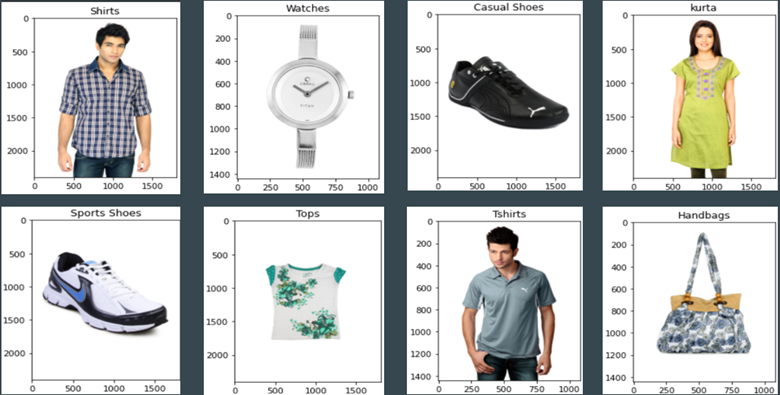
\includegraphics[width=80mm]{fig_2.png}
    \caption{Product image data overview}
    \label{fig:12}
\end{figure}

\textbf{Data Preprocessing}: The given images from our dataset are of different dimensions. But neural networks especially CNN require the input images to have the same size or dimension. Since we are using the pre-trained Xception model architecture, the input image is required to have the shape (299, 299, d) where d is the number of channels for the given image. So, for preprocessing we resized all the images to height and weight of 299 and 299 pixels respectively. 

To increase the model’s performance, we also performed data augmentation techniques such as horizontal and vertical flipping. All these images along with the original 12k images were fed to train the CNN model.

\subsection{Results}
In this section we discuss our results for the image classification model and the recommendation outputs from the CNN.

\textbf{Product Category Classification}: We train the Xception model using pre-trained weights from the ImageNet dataset and freeze the top layers while training the lower layers to fine-tune the model for our purpose of product classification model\cite{exception}. To avoid the problem of over-fitting, we used callbacks such as EarlyStopping and ModelCheckpoint\cite{chollet2015keras}. We also used an exponential learning rate which would help the model perform better when it comes to product category classification. The model was trained for 3 epochs in total with a batch size of 64. Here are the results of the product classification using CNN:

\begin{figure}[!h]
    \centering
    % \captionsetup{justification=centering,margin=2cm}
    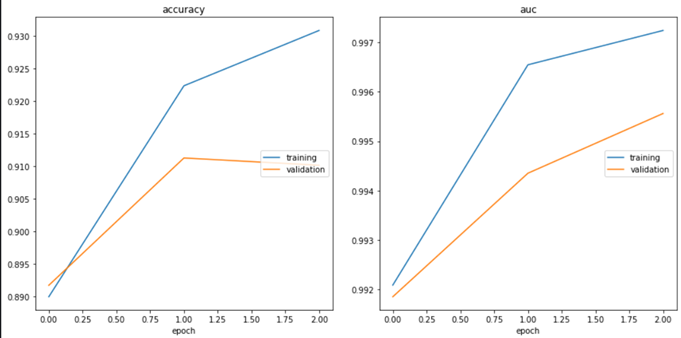
\includegraphics[width=90mm]{fig_3.png}
    \caption{Plot of Accuracy and loss function metrics during Training}
    \label{fig:13}
\end{figure}

\begin{figure}[!h]
    \centering
    % \captionsetup{justification=centering,margin=2cm}
    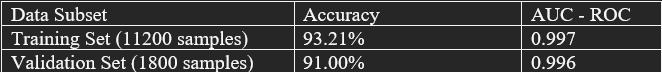
\includegraphics[width=90mm]{fig_8.png}
    \caption{Model Evaluation table}
    \label{fig:13}
\end{figure}

\textbf{Product Recommendation}: We used the CNN classifier as a feature extractor to get the image embeddings for all the given images and for the new input images. The feature embedding vectors form a matrix of the size    n * 2048 (rows * columns). Given an input image, the feature extractor extracts the image embeddings and passes it through the Annoy to get similar image product recommendations. Here are a couple of output results from the two-stage recommendation system:

\begin{figure}[!h]
    \centering
    % \captionsetup{justification=centering,margin=2cm}
    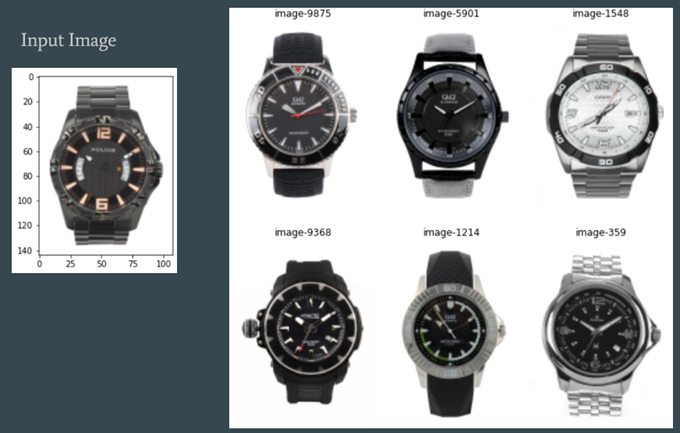
\includegraphics[width=80mm]{fig_5.png}
    \caption{Output from our two-stage fashion recommendation system given a watch image as an input.}
    \label{fig:14}
\end{figure}

\begin{figure}[!h]
    \centering
    % \captionsetup{justification=centering,margin=2cm}
    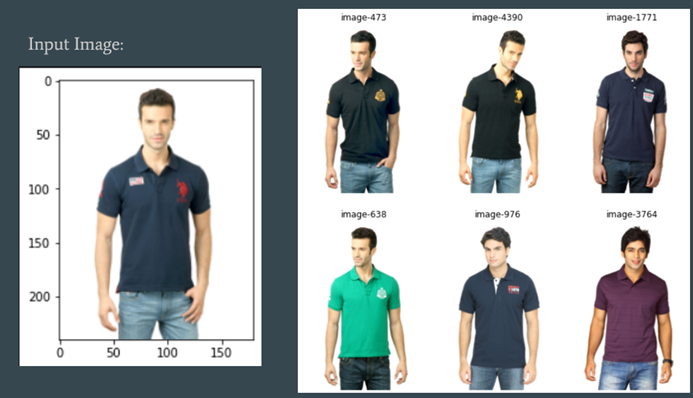
\includegraphics[width=80mm]{fig_6.png}
    \caption{Output from our two-stage fashion recommendation system given a t-shirt image as an input}
    \label{fig:15}
\end{figure}


\section{Conclusion and Future Work}
We presented our two-stage framework doing image similarity. In the first stage,
we trained a CNN model using transfer learning to classify a given product image into one of the 8 categories. In the second stage, the image embeddings obtained from the CNN model were used as a database and a search space for the Approximate Nearest Neighbor algorithm Annoy. The two-stage implementation of our proposed fashion recommendation system was able to recommend similar product images to a given product image. The proposed recommendation system can be used by the e-commerce websites to provide live recommendations when a user is viewing a product or as a search engine where a user can upload an image and similar products available for purchase can be displayed.

Future work includes improving the image embeddings by concatenating the item description with the visual appearance and building a feature extractor using a LSTM model and a CNN model to better understand more low-level features from the data to provide recommendations. This approach can be extended to an unsupervised setting where we don’t have labeled data for the product categories and an auto-encoder can be used to extract the visual features. Also, a hybrid combination of image-based and either collaborative-based or content-based recommendation system for fashion products could be explored.

\section{Work division}
\textbf{Kushajveer Singh (811777259)}

\textbf{Vipul Shinde (811312777)}

{\small
\bibliographystyle{ieee_fullname}
\bibliography{egbib}
}

\end{document}
